\documentclass[10pt,a4paper]{article}

%double si on veut une version prof et une version élève. simple si on veut une seule version.
\newcommand{\buildmode}{simple}

\InputIfFileExists{version.tex}{}{}
% Version (définie par le script)
\providecommand{\version}{eleve}

\usepackage{feuilleinterro}

%%%à modifier à chaque fois

\renewcommand{\niveau}{1G}
\renewcommand{\chapitre}{Fonctions, généralités}
\renewcommand{\numchap}{0}
\renewcommand{\theme}{Fonctions}

%%%titre "CORRECTION" au lieu de "INTERROGATION", sans les champs Nom/Prénom
\renewcommand{\interroversion}[1]{
    \noindent\textbf{\niveau}

    \vspace{-0.5cm}
    \begin{center}
        \textbf{\large CORRECTION -- \chapitre}
    \end{center}

    \vspace{0.1cm}
}

\begin{document}

% =========================================================
% PAGE 1 : VERSION A
% =========================================================

\interroversion{A}

\textbf{Exercice 1 -- Image par une fonction polynôme du second degré \hfill /1}

Soit \(g\) la fonction définie sur \(\mathbb{R}\) par \(g(x)=2x^2-3x-1\). Calculer \(g(-2)\).

On remplace \(x\) par \(-2\) :
\[
\begin{aligned}
g(-2) &= 2\times(-2)^2-3\times(-2)-1\\
      &= 2\times4-3\times(-2)-1\\
      &= 8+6-1\\
      &= 13.
\end{aligned}
\]

\textbf{Exercice 2 -- Signe d'un produit de fonctions affines \hfill /4}

On considère les fonctions affines \(f\) et \(g\) définies sur \(\mathbb{R}\) par
\[
f(x)=2x-3 \qquad\text{et}\qquad g(x)=-x+4,
\]
ainsi que la fonction \(h\) définie sur \(\mathbb{R}\) par \(h(x)=f(x)\times g(x)\).

\begin{enumerate}
\item Donner les représentations graphiques approximatives des fonctions \(f\) et \(g\).

\begin{center}
\begin{minipage}{2.6cm}
\centering
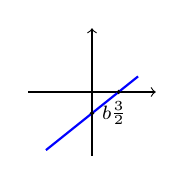
\begin{tikzpicture}[scale=0.45]
\draw[->] (-1.8,0) -- (1.8,0);
\draw[->] (0,-1.8) -- (0,1.8);
\draw[thick,blue] (-1.3,-1.64) -- (1.3,0.44);
\filldraw (0,-0.6) circle (1.2pt) node[right]{\scriptsize \(b\)};
\filldraw (0.75,0) circle (1.2pt) node[below]{\scriptsize \(\frac{3}{2}\)};
\end{tikzpicture}\\[2pt]
{\scriptsize \textcolor{blue}{\(f\)} : \(a=2>0\), \(b=-3\)}
\end{minipage}
\hspace{0.3cm}
\begin{minipage}{2.6cm}
\centering
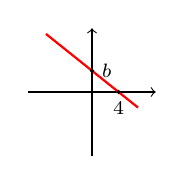
\begin{tikzpicture}[scale=0.45]
\draw[->] (-1.8,0) -- (1.8,0);
\draw[->] (0,-1.8) -- (0,1.8);
\draw[thick,red] (-1.3,1.64) -- (1.3,-0.44);
\filldraw (0,0.6) circle (1.2pt) node[right]{\scriptsize \(b\)};
\filldraw (0.75,0) circle (1.2pt) node[below]{\scriptsize \(4\)};
\end{tikzpicture}\\[2pt]
{\scriptsize \textcolor{red}{\(g\)} : \(a=-1<0\), \(b=4\)}
\end{minipage}
\end{center}

\begin{center}
\begin{minipage}{0.48\linewidth}
\(f\) a pour coefficient directeur \(a=2>0\) : \(f\) est croissante.
\[
\begin{aligned}
f(x)&>0\\
2x-3&>0 &\scriptstyle(+3)\\
2x&>3 &\scriptstyle(\div 2)\\
x&>\frac{3}{2}.
\end{aligned}
\]
\end{minipage}
\hfill
\begin{minipage}{0.48\linewidth}
\(g\) a pour coefficient directeur \(a=-1<0\) : \(g\) est décroissante.
\[
\begin{aligned}
g(x)&>0\\
-x+4&>0 &\scriptstyle(-4)\\
-x&>-4 &\scriptstyle(\div(-1))\\
x&<4.
\end{aligned}
\]
\end{minipage}
\end{center}

\item En déduire le tableau de signes de \(h\) sur \(\mathbb{R}\).

Sur chaque intervalle, le signe de \(h(x)=f(x)\times g(x)\) s'obtient en multipliant le signe de \(f(x)\) par celui de \(g(x)\) (règle des signes d'un produit).

\begin{center}
\begin{tikzpicture}
\tkzTabInit[lgt=1.1,espcl=1.3]{\(x\) /1, \(f(x)\) /1, \(g(x)\) /1, \(h(x)\) /1}{\(-\infty\),\(\frac{3}{2}\),\(4\),\(+\infty\)}
\tkzTabLine{,-,0,+,,+,}
\tkzTabLine{,+,,+,0,-,}
\tkzTabLine{,-,0,+,0,-,}
\end{tikzpicture}
\end{center}

\item Décrire le tableau de signes obtenu.

\(h\) est strictement négative sur \(\left]-\infty;\frac{3}{2}\right[\), nulle en \(\frac{3}{2}\), strictement positive sur \(\left]\frac{3}{2};4\right[\), nulle en \(4\), puis strictement négative sur \(]4;+\infty[\).
\end{enumerate}

\newpage

% =========================================================
% PAGE 2 : VERSION B
% =========================================================

\interroversion{B}

\textbf{Exercice 1 -- Image par une fonction polynôme du second degré \hfill /1}

Soit \(g\) la fonction définie sur \(\mathbb{R}\) par \(g(x)=x^2-4x+2\). Calculer \(g(-3)\).

On remplace \(x\) par \(-3\) :
\[
\begin{aligned}
g(-3) &= (-3)^2-4\times(-3)+2\\
      &= 9-4\times(-3)+2\\
      &= 9+12+2\\
      &= 23.
\end{aligned}
\]

\textbf{Exercice 2 -- Signe d'un produit de fonctions affines \hfill /4}

On considère les fonctions affines \(f\) et \(g\) définies sur \(\mathbb{R}\) par
\[
f(x)=-3x+6 \qquad\text{et}\qquad g(x)=x+1,
\]
ainsi que la fonction \(h\) définie sur \(\mathbb{R}\) par \(h(x)=f(x)\times g(x)\).

\begin{enumerate}
\item Donner les représentations graphiques approximatives des fonctions \(f\) et \(g\).

\begin{center}
\begin{minipage}{2.6cm}
\centering
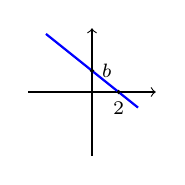
\begin{tikzpicture}[scale=0.45]
\draw[->] (-1.8,0) -- (1.8,0);
\draw[->] (0,-1.8) -- (0,1.8);
\draw[thick,blue] (-1.3,1.64) -- (1.3,-0.44);
\filldraw (0,0.6) circle (1.2pt) node[right]{\scriptsize \(b\)};
\filldraw (0.75,0) circle (1.2pt) node[below]{\scriptsize \(2\)};
\end{tikzpicture}\\[2pt]
{\scriptsize \textcolor{blue}{\(f\)} : \(a=-3<0\), \(b=6\)}
\end{minipage}
\hspace{0.3cm}
\begin{minipage}{2.6cm}
\centering
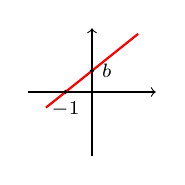
\begin{tikzpicture}[scale=0.45]
\draw[->] (-1.8,0) -- (1.8,0);
\draw[->] (0,-1.8) -- (0,1.8);
\draw[thick,red] (-1.3,-0.44) -- (1.3,1.64);
\filldraw (0,0.6) circle (1.2pt) node[right]{\scriptsize \(b\)};
\filldraw (-0.75,0) circle (1.2pt) node[below]{\scriptsize \(-1\)};
\end{tikzpicture}\\[2pt]
{\scriptsize \textcolor{red}{\(g\)} : \(a=1>0\), \(b=1\)}
\end{minipage}
\end{center}

\begin{center}
\begin{minipage}{0.48\linewidth}
\(f\) a pour coefficient directeur \(a=-3<0\) : \(f\) est décroissante.
\[
\begin{aligned}
f(x)&>0\\
-3x+6&>0 &\scriptstyle(-6)\\
-3x&>-6 &\scriptstyle(\div(-3))\\
x&<2.
\end{aligned}
\]
\end{minipage}
\hfill
\begin{minipage}{0.48\linewidth}
\(g\) a pour coefficient directeur \(a=1>0\) : \(g\) est croissante.
\[
\begin{aligned}
g(x)&>0\\
x+1&>0 &\scriptstyle(-1)\\
x&>-1.
\end{aligned}
\]
\end{minipage}
\end{center}

\item En déduire le tableau de signes de \(h\) sur \(\mathbb{R}\).

Sur chaque intervalle, le signe de \(h(x)=f(x)\times g(x)\) s'obtient en multipliant le signe de \(f(x)\) par celui de \(g(x)\) (règle des signes d'un produit).

\begin{center}
\begin{tikzpicture}
\tkzTabInit[lgt=1.1,espcl=1.3]{\(x\) /1, \(f(x)\) /1, \(g(x)\) /1, \(h(x)\) /1}{\(-\infty\),\(-1\),\(2\),\(+\infty\)}
\tkzTabLine{,+,,+,0,-,}
\tkzTabLine{,-,0,+,,+,}
\tkzTabLine{,-,0,+,0,-,}
\end{tikzpicture}
\end{center}

\item Décrire le tableau de signes obtenu.

\(h\) est strictement négative sur \(]-\infty;-1[\), nulle en \(-1\), strictement positive sur \(]-1;2[\), nulle en \(2\), puis strictement négative sur \(]2;+\infty[\).
\end{enumerate}

\newpage

% =========================================================
% PAGE 3 : VERSION C
% =========================================================

\interroversion{C}

\textbf{Exercice 1 -- Image par une fonction polynôme du second degré \hfill /1}

Soit \(g\) la fonction définie sur \(\mathbb{R}\) par \(g(x)=x^2+5x-4\). Calculer \(g(-3)\).

On remplace \(x\) par \(-3\) :
\[
\begin{aligned}
g(-3) &= (-3)^2+5\times(-3)-4\\
      &= 9+5\times(-3)-4\\
      &= 9-15-4\\
      &= -10.
\end{aligned}
\]

\textbf{Exercice 2 -- Signe d'un produit de fonctions affines \hfill /4}

On considère les fonctions affines \(f\) et \(g\) définies sur \(\mathbb{R}\) par
\[
f(x)=4x-2 \qquad\text{et}\qquad g(x)=-2x-4,
\]
ainsi que la fonction \(h\) définie sur \(\mathbb{R}\) par \(h(x)=f(x)\times g(x)\).

\begin{enumerate}
\item Donner les représentations graphiques approximatives des fonctions \(f\) et \(g\).

\begin{center}
\begin{minipage}{2.6cm}
\centering
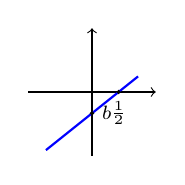
\begin{tikzpicture}[scale=0.45]
\draw[->] (-1.8,0) -- (1.8,0);
\draw[->] (0,-1.8) -- (0,1.8);
\draw[thick,blue] (-1.3,-1.64) -- (1.3,0.44);
\filldraw (0,-0.6) circle (1.2pt) node[right]{\scriptsize \(b\)};
\filldraw (0.75,0) circle (1.2pt) node[below]{\scriptsize \(\frac{1}{2}\)};
\end{tikzpicture}\\[2pt]
{\scriptsize \textcolor{blue}{\(f\)} : \(a=4>0\), \(b=-2\)}
\end{minipage}
\hspace{0.3cm}
\begin{minipage}{2.6cm}
\centering
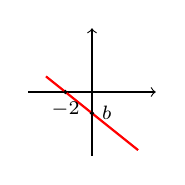
\begin{tikzpicture}[scale=0.45]
\draw[->] (-1.8,0) -- (1.8,0);
\draw[->] (0,-1.8) -- (0,1.8);
\draw[thick,red] (-1.3,0.44) -- (1.3,-1.64);
\filldraw (0,-0.6) circle (1.2pt) node[right]{\scriptsize \(b\)};
\filldraw (-0.75,0) circle (1.2pt) node[below]{\scriptsize \(-2\)};
\end{tikzpicture}\\[2pt]
{\scriptsize \textcolor{red}{\(g\)} : \(a=-2<0\), \(b=-4\)}
\end{minipage}
\end{center}

\begin{center}
\begin{minipage}{0.48\linewidth}
\(f\) a pour coefficient directeur \(a=4>0\) : \(f\) est croissante.
\[
\begin{aligned}
f(x)&>0\\
4x-2&>0 &\scriptstyle(+2)\\
4x&>2 &\scriptstyle(\div 4)\\
x&>\frac{1}{2}.
\end{aligned}
\]
\end{minipage}
\hfill
\begin{minipage}{0.48\linewidth}
\(g\) a pour coefficient directeur \(a=-2<0\) : \(g\) est décroissante.
\[
\begin{aligned}
g(x)&>0\\
-2x-4&>0 &\scriptstyle(+4)\\
-2x&>4 &\scriptstyle(\div(-2))\\
x&<-2.
\end{aligned}
\]
\end{minipage}
\end{center}

\item En déduire le tableau de signes de \(h\) sur \(\mathbb{R}\).

Sur chaque intervalle, le signe de \(h(x)=f(x)\times g(x)\) s'obtient en multipliant le signe de \(f(x)\) par celui de \(g(x)\) (règle des signes d'un produit).

\begin{center}
\begin{tikzpicture}
\tkzTabInit[lgt=1.1,espcl=1.3]{\(x\) /1, \(f(x)\) /1, \(g(x)\) /1, \(h(x)\) /1}{\(-\infty\),\(-2\),\(\frac{1}{2}\),\(+\infty\)}
\tkzTabLine{,-,,-,0,+,}
\tkzTabLine{,+,0,-,,-,}
\tkzTabLine{,-,0,+,0,-,}
\end{tikzpicture}
\end{center}

\item Décrire le tableau de signes obtenu.

\(h\) est strictement négative sur \(]-\infty;-2[\), nulle en \(-2\), strictement positive sur \(\left]-2;\frac{1}{2}\right[\), nulle en \(\frac{1}{2}\), puis strictement négative sur \(\left]\frac{1}{2};+\infty\right[\).
\end{enumerate}

\newpage

% =========================================================
% PAGE 4 : VERSION D
% =========================================================

\interroversion{D}

\textbf{Exercice 1 -- Image par une fonction polynôme du second degré \hfill /1}

Soit \(g\) la fonction définie sur \(\mathbb{R}\) par \(g(x)=3x^2-x+2\). Calculer \(g(-1)\).

On remplace \(x\) par \(-1\) :
\[
\begin{aligned}
g(-1) &= 3\times(-1)^2-(-1)+2\\
      &= 3\times1-(-1)+2\\
      &= 3+1+2\\
      &= 6.
\end{aligned}
\]

\textbf{Exercice 2 -- Signe d'un produit de fonctions affines \hfill /4}

On considère les fonctions affines \(f\) et \(g\) définies sur \(\mathbb{R}\) par
\[
f(x)=-x+3 \qquad\text{et}\qquad g(x)=3x+6,
\]
ainsi que la fonction \(h\) définie sur \(\mathbb{R}\) par \(h(x)=f(x)\times g(x)\).

\begin{enumerate}
\item Donner les représentations graphiques approximatives des fonctions \(f\) et \(g\).

\begin{center}
\begin{minipage}{2.6cm}
\centering
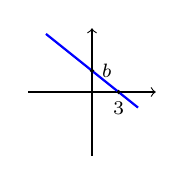
\begin{tikzpicture}[scale=0.45]
\draw[->] (-1.8,0) -- (1.8,0);
\draw[->] (0,-1.8) -- (0,1.8);
\draw[thick,blue] (-1.3,1.64) -- (1.3,-0.44);
\filldraw (0,0.6) circle (1.2pt) node[right]{\scriptsize \(b\)};
\filldraw (0.75,0) circle (1.2pt) node[below]{\scriptsize \(3\)};
\end{tikzpicture}\\[2pt]
{\scriptsize \textcolor{blue}{\(f\)} : \(a=-1<0\), \(b=3\)}
\end{minipage}
\hspace{0.3cm}
\begin{minipage}{2.6cm}
\centering
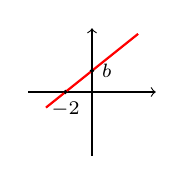
\begin{tikzpicture}[scale=0.45]
\draw[->] (-1.8,0) -- (1.8,0);
\draw[->] (0,-1.8) -- (0,1.8);
\draw[thick,red] (-1.3,-0.44) -- (1.3,1.64);
\filldraw (0,0.6) circle (1.2pt) node[right]{\scriptsize \(b\)};
\filldraw (-0.75,0) circle (1.2pt) node[below]{\scriptsize \(-2\)};
\end{tikzpicture}\\[2pt]
{\scriptsize \textcolor{red}{\(g\)} : \(a=3>0\), \(b=6\)}
\end{minipage}
\end{center}

\begin{center}
\begin{minipage}{0.48\linewidth}
\(f\) a pour coefficient directeur \(a=-1<0\) : \(f\) est décroissante.
\[
\begin{aligned}
f(x)&>0\\
-x+3&>0 &\scriptstyle(-3)\\
-x&>-3 &\scriptstyle(\div(-1))\\
x&<3.
\end{aligned}
\]
\end{minipage}
\hfill
\begin{minipage}{0.48\linewidth}
\(g\) a pour coefficient directeur \(a=3>0\) : \(g\) est croissante.
\[
\begin{aligned}
g(x)&>0\\
3x+6&>0 &\scriptstyle(-6)\\
3x&>-6 &\scriptstyle(\div 3)\\
x&>-2.
\end{aligned}
\]
\end{minipage}
\end{center}

\item En déduire le tableau de signes de \(h\) sur \(\mathbb{R}\).

Sur chaque intervalle, le signe de \(h(x)=f(x)\times g(x)\) s'obtient en multipliant le signe de \(f(x)\) par celui de \(g(x)\) (règle des signes d'un produit).

\begin{center}
\begin{tikzpicture}
\tkzTabInit[lgt=1.1,espcl=1.3]{\(x\) /1, \(f(x)\) /1, \(g(x)\) /1, \(h(x)\) /1}{\(-\infty\),\(-2\),\(3\),\(+\infty\)}
\tkzTabLine{,+,,+,0,-,}
\tkzTabLine{,-,0,+,,+,}
\tkzTabLine{,-,0,+,0,-,}
\end{tikzpicture}
\end{center}

\item Décrire le tableau de signes obtenu.

\(h\) est strictement négative sur \(]-\infty;-2[\), nulle en \(-2\), strictement positive sur \(]-2;3[\), nulle en \(3\), puis strictement négative sur \(]3;+\infty[\).
\end{enumerate}

\end{document}
